% -*- coding: utf-8 -*-
\documentclass{article}
\usepackage{listings}
\usepackage{ctex}
\usepackage{graphicx}
\usepackage[a4paper, body={18cm,22cm}]{geometry}
\usepackage{amsmath,amssymb,amstext,wasysym,enumerate,graphicx}
\usepackage{float,abstract,booktabs,indentfirst,amsmath}
\usepackage{array}
\usepackage{booktabs} %调整表格线与上下内容的间隔
\usepackage{multirow}
\usepackage{url}
\usepackage{diagbox}
\renewcommand\arraystretch{1.4}
\usepackage{indentfirst}
\setlength{\parindent}{2em}

\usepackage{listings}
\usepackage{xcolor}
\lstset{
    numbers=left, 
    numberstyle= \tiny, 
    keywordstyle= \color{ blue!70},
    commentstyle= \color{red!50!green!50!blue!50}, 
    frame=shadowbox, % 阴影效果
    rulesepcolor= \color{ red!20!green!20!blue!20} ,
    escapeinside=``, % 英文分号中可写入中文
    xleftmargin=2em,xrightmargin=2em, aboveskip=1em,
    basicstyle=\footnotesize,
    framexleftmargin=2em
} 


\geometry{left=2.8cm,right=2.2cm,top=2.5cm,bottom=2.5cm}
%\geometry{left=3.18cm,right=3.18cm,top=2.54cm,bottom=2.54cm}

\graphicspath{{figures/}}

\title{\heiti 深度学习方法与实践 实验一}

\begin{document}
    \maketitle
    %\tableofcontents
    
    \begin{center}
        %\LARGE{{\textbf{\heiti 实验一 远程过程调用中间件及数据访问中间件}}}
        %\newline
        %\newline
        %\date{2019年4月2日}
        \begin{table}[H]
            \centering
            \begin{tabular}{p{2cm}p{4cm}<{\centering}p{2cm}p{4cm}<{\centering}}
                年\quad 级: & 2020级 & 学\qquad 号:   & 2016012963 \\ \cline{2-2} \cline{4-4} 
                姓\quad 名: & 董佩杰      & 指导老师: & 牛新        \\ \cline{2-2} \cline{4-4} 
            \end{tabular}
        \end{table}
    \end{center}
    
    \section{用OpenCV画飞机}
    
    	\subsection{要求}
    		\begin{itemize}
    			
    			\item 用python中的opencv库画3种飞机,并经过旋转扩充,标注关键点,形成飞机飞机分类与关键点预测数据集 "AIRPLANES"。
    			\item 飞机颜色要求正确:椭圆用蓝色,长方形用红色,三角形用黄色,并且椭圆机身在最顶层,盖住机翼和尾翼。
    			\item 按照要求打包和提交材料。
    			
    		\end{itemize}
    	
    	\subsection{飞机的结果}
    	
    		以下是按照格式进行旋转的图片,分别对应的是三个类:“AIRBUS”、“FIGHTER”和“UAV”
    		
    		
		    \begin{figure}[h]
	   			% 一个2*2图片的排列
	   			\begin{minipage}[h]{0.3\linewidth}
	   				\centering
	   				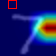
\includegraphics[width=0.8\textwidth]{./1.jpg}
	   				\caption{AIRBUS类别对应的图片和标签}
	   			\end{minipage}
	   			\begin{minipage}[h]{0.3\linewidth}
	   				\centering
	   				\includegraphics[width=0.8\textwidth]{./2.jpg}
	   				\caption{FIGHTER类别对应的图片和标签}
	   			\end{minipage}
   			   	\begin{minipage}[h]{0.3\linewidth}
		   			\centering
		   			\includegraphics[width=0.8\textwidth]{./3.jpg}
		   			\caption{UAV类别对应的图片和标签}
		   		\end{minipage}   		
    		\end{figure}
    	
    	
    		\begin{figure}[h]
    			% 一个2*2图片的排列
    			\begin{minipage}[h]{0.3\linewidth}
    				\centering
    				\includegraphics[width=0.8\textwidth]{./4.jpg}
    				\caption{AIRBUS类别对应的标注结果}
    			\end{minipage}
    			\begin{minipage}[h]{0.3\linewidth}
    				\centering
    				\includegraphics[width=0.8\textwidth]{./5.jpg}
    				\caption{FIGHTER类别对应的标注结果}
    			\end{minipage}
    			\begin{minipage}[h]{0.3\linewidth}
    				\centering
    				\includegraphics[width=0.8\textwidth]{./6.jpg}
    				\caption{UAV类别对应的标注结果}
    			\end{minipage}   		
    		\end{figure}
    	
    	最终文件内容为:
    	
    	\begin{figure}[h]
    		\centering
    		\includegraphics[width=6cm]{./7.jpg}
    		\caption{以UAV为例的标注文件内容} \label{fig:aa}
    	\end{figure}
    	
    	\subsection{思路}
    	
    	实验的要求是使用opencv来完善代码中没有构建完成的部分,并且提供了“AIRBUS”类别的样例。按照样例可以很快完成剩余两个类的构建。在构建过程中需要注意两个地方:
    	
    	(1) 画图的顺序,椭圆代表的机身是需要最后画的。
    	
    	(2) cv2.rectangle的用法,这个方法需要注意的是使用的坐标是矩形左上角坐标和右下角坐标。并且由于rectangle有两个构造函数,其中一个不是坐标,而是rect参数,这时候最好指名使用的是哪个构造函数:
    	
\begin{lstlisting}
img = cv2.rectangle(
	img=img,
	pt1=tuple(np.array(LP_UAV['BLwing']) - np.array([0, WIDTH_WING])),
	pt2=tuple(LP_UAV['BRwing']),
	color=(0, 0, 255),
	thickness=-1)
\end{lstlisting}

		三个构件图片的函数写完以后,开始完善\textbf{rotate\_anno}函数,首先要搞清楚三个参数:savepath代表保存的txt标注文件;angle代表旋转的角度,p\_sets不是特别明显,但是可以通过下面的提示得到这是字典,所以就直接通过字典访问得到对应的坐标即可。
\begin{lstlisting}
def rotate_anno(savepath, angle, p_sets):
	f_save = open(savepath, 'w')
	for p in p_sets:
		#-------------to do-----------------------
		x = p_sets[p][0]
		y = p_sets[p][1]
		#-------------to do-----------------------
		x, y = rotate_onepoint(x, y, angle)
		newline = str(p) + ' ' + str(x) + ' ' + str(y) + '\n'
		f_save.writelines(newline)
	f_save.close()	
\end{lstlisting}
    	
    	接下来就是\textbf{make\_data}函数,在题目中已经有提示,只需要注意文件命名规则等细节即可完成。代码如下:
    	
\begin{lstlisting}
def make_data(PATH_DATA_SET, name_data, num):
	#-------------to do-----------------------
	PATH_DATA = osp.join(PATH_DATA_SET, name_data)
	if not osp.exists(PATH_DATA):
		os.makedirs(PATH_DATA)
	#-------------to do-----------------------
	if name_data == 'AIRBUS':
		img = draw_airbus()
		p_sets = LP_AIRBUS
	elif name_data == 'FIGHTER':
		img = draw_fighter()
		p_sets = LP_FIGHTER
	elif name_data == 'UAV':
		img = draw_uav()
		p_sets = LP_UAV
	else:
		print('wrong data')
	
	
	#-------------to do-----------------------
	for i in range(num):
		angle = random.randint(0, 359)
		rotate_anno(osp.join(PATH_DATA, name_data + "_%d.txt" % angle), angle, p_sets)
		matRotate = cv2.getRotationMatrix2D(
		(SIZE_IMG * 0.5, SIZE_IMG * 0.5), angle,1) 
		img_r = cv2.warpAffine(img, matRotate, (SIZE_IMG, SIZE_IMG))
		cv2.imwrite(osp.join(PATH_DATA, name_data + "_%d.jpg" % angle), img_r)
	
\end{lstlisting}
    
    \section{拟合余弦函数}
       
		\subsection{要求}
		
		假设有函数y = cos(ax + b), 其中a为学号前两位,b为学号最后两位。首先从此函数中以相同步长(点与点之间在x轴上距离相同),在0<(ax+b)<2pi范围内,采样出2000个点,然后利用采样的2000个点作为特征点进行三次函数拟合。
		
		\subsection{拟合结果}
		
		主要是通过np.polyfit函数进行三次拟合。代码如下:

\begin{lstlisting}
# 学号: 2016012963
# 函数:y = cos(20x+63)
import math
import numpy as np
import matplotlib.pyplot as plt


def func(x):
	return math.cos(20 * x + 63)

if __name__ == "__main__":
	x = np.linspace(-63.0 / 20, float(2 * math.pi - 63) / 20, 2000)
	y = [func(i) for i in x]
	
	f1 = np.polyfit(x, y, 3)
	p = np.poly1d(f1)
	
	y2 = p(x)
	
	plt.scatter(x, y)
	plt.scatter(x, y2)
	plt.show()
\end{lstlisting}
		
		下面是可视化结果:
		
		\begin{figure}[H]
			\centering
			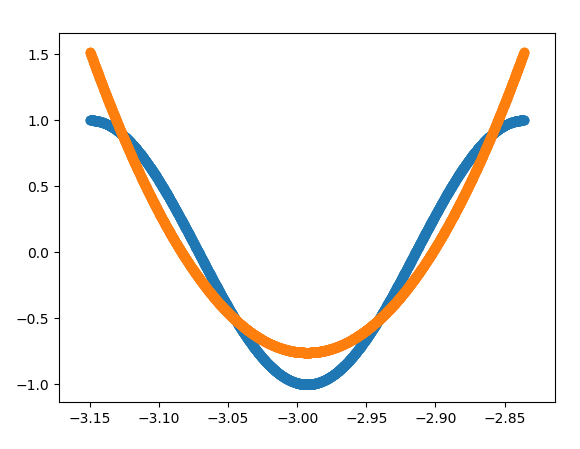
\includegraphics[width=0.5\linewidth]{8}
			\caption{用三次函数模拟余弦函数的结果}
			\label{fig:8}
		\end{figure}      
    
\end{document}

%%%%%%%%%%%%%%%%%%%%%%%%%%%%Library%%%%%%%%%%%%%%%%%%%%%%%%%%%%%%%%%%%%%%%

% 1. 脚注用法
    LaTeX\footnote{Latex is Latex} is a good software

%2. 强调
    \emph{center of percussion} %[Brody 1986], %\lipsum[5]

%3. 随便生成一段话
    \lipsum[4]

%4. 列条目
    \begin{itemize}
    \item the angular velocity of the bat,
    \item the velocity of the ball, and
    \item the position of impact along the bat.
    \end{itemize}

%5. 表格用法
    \begin{table}[h]
    \centering  
    \begin{tabular}{c|cc}
        \hline
        年份 & \multicolumn{2}{c}{指标}\\
        \hline
        2017 & 0.9997 & 0.0555 \\
        2018 & 0.9994 & 0      \\
        2019 & 0.9993 & 0      \\
        \hline
    \end{tabular}
    \caption{NAME}\label{SIGN}
    \end{table}

    \begin{center}
        \begin{tabular}{c|cclcrcc}
            \hline
            Year & theta & $S_1^-$ & $S_2^-$ & $S_3^-$ & $S_4^+$ & $S_5^+$ & $S_6^+$ \\%表格标题
            \hline
            2016 & 1      & 0      & 0 & 0.0001 & 0      & 0      & 0 \\
            2017 & 0.9997 & 0.0555 & 0 & 0.2889 & 0.1844 & 0.463  & 0 \\
            2018 & 0.9994 & 0      & 0 & 0.0012 & 0.3269 & 0.7154 & 0 \\
            2019 & 0.9993 & 0      & 0 & 0      & 0.4325 & 1.0473 & 0 \\
            2020 & 0.9991 & 0      & 0 & 0      & 0.5046 & 1.2022 & 0 \\
            2021 & 0.999  & 0      & 0 & 0      & 0.5466 & 1.2827 & 0 \\
            2022 & 0.9989 & 0.0017 & 0 & 0.3159 & 0.562  & 1.2995 & 0 \\
            2023 & 0.9989 & 0      & 0 & 0.0109 & 0.5533 & 1.2616 & 0 \\
            2024 & 0.9989 & 0      & 0 & 0      & 0.5232 & 1.1769 & 0 \\
            2025 & 0.9989 & 0      & 0 & 0.1009 & 0.4738 & 1.0521 & 0 \\
            2026 & 0.9991 & 0      & 0 & 0      & 0.4071 & 0.8929 & 0 \\
            2027 & 0.9992 & 0.0004 & 0 & 0.1195 & 0.3248 & 0.7042 & 0 \\
            2028 & 0.9994 & 0.0164 & 0 & 0.046  & 0.2287 & 0.4902 & 0 \\
            2029 & 0.9997 & 0      & 0 & 0.0609 & 0.12   & 0.2545 & 0 \\
            2030 & 1      & 0      & 0 & 0      & 0      & 0      & 0 \\
            \hline
        \end{tabular}
    \end{center}

%6. 数学公式
    \begin{equation}
        a^2 = a * a\label{aa}
    \end{equation}
    
    \[
    \begin{pmatrix}{*{20}c}
    {a_{11} } & {a_{12} } & {a_{13} }  \\
    {a_{21} } & {a_{22} } & {a_{23} }  \\
    {a_{31} } & {a_{32} } & {a_{33} }  \\
    \end{pmatrix}
    = \frac{{Opposite}}{{Hypotenuse}}\cos ^{ - 1} \theta \arcsin \theta
    \]
    
    \[
    p_{j}=\begin{cases} 0,&\text{if $j$ is odd}\\
    r!\,(-1)^{j/2},&\text{if $j$ is even}
    \end{cases}
    \]
    
    
    \[
    \arcsin \theta  =
    \mathop{{\int\!\!\!\!\!\int\!\!\!\!\!\int}\mkern-31.2mu
        \bigodot}\limits_\varphi
    {\mathop {\lim }\limits_{x \to \infty } \frac{{n!}}{{r!\left( {n - r}
                \right)!}}} \eqno (1)
    \]

%7. 双图并行
    \begin{figure}[h]
        % 一个2*2图片的排列
        \begin{minipage}[h]{0.5\linewidth}
            \centering
            \includegraphics[width=0.8\textwidth]{./figures/0.jpg}
            \caption{Figure example 2}
        \end{minipage}
        \begin{minipage}[h]{0.5\linewidth}
            \centering
            \includegraphics[width=0.8\textwidth]{./figures/0.jpg}
            \caption{Figure example 3}
        \end{minipage}
    \end{figure}

%8. 单张图片部分
    \begin{figure}[h]
        %\small
        \centering
        \includegraphics[width=12cm]{./figures/mcmthesis-aaa.eps}
        \caption{Figure example 1} \label{fig:aa}
    \end{figure}

%%%%%%%%%%%%%%%%%%%%%%%%%%%%%%%%%%%%%%%%%%%%%%%%%%%%%%%%%%%%%%%%%%%%%%%%%%%%%
\begin{minipage}{0.5\linewidth}
    \begin{tabular}{|c|c|c|}
        \hline
        \multicolumn{2}{|c|}{\multirow{2}{*}{合并}}&测试\\
        \cline{3-3}
        \multicolumn{2}{|c|}{}& 0.9997  \\
        \hline
        2019 & 0.9993 & 0 \\
        \hline
    \end{tabular}
\end{minipage}

\begin{minipage}{0.5\linewidth}
    \begin{tabular}{c|ccc}
        \hline
        年份 & \multicolumn{3}{c}{指标}\\
        \hline
        \multirow{3}{*}{合并}&2017 & 0.9997 & 0.0555 \\
        &2018 & 0.9994 & 0      \\
        &2019 & 0.9993 & 0      \\
        \hline
    \end{tabular}
\end{minipage}



    \begin{table}[h]
    \centering  
    \begin{Large}
        \begin{tabular}{p{4scm} p{8cm} < {\centering}}
            \hline
            院\qquad 系: & 信息工程学院 \\
            \hline
            团队名称: & PlantBook Team \\
            \hline
            分\qquad 组: & 第0组1号 \\
            \hline
            日\qquad 期: & 2017年10月28日 \\
            \hline
            指导教师: & 吱吱吱\\
            \hline
        \end{tabular}
    \end{Large}
\end{table}


\ctexset{
    section={
        format+=\heiti \raggedright,
        name={,、},
        number=\chinese{section},
        beforeskip=1.0ex plus 0.2ex minus .2ex,
        afterskip=1.0ex plus 0.2ex minus .2ex,
        aftername=\hspace{0pt}
    },
}

    \begin{table}[h]
    \centering
    \begin{Large}
        \begin{tabular}{p{3cm} p{7cm}<{\centering}}
            院  \qquad  系: & ***          \\ \cline{2-2}
        \end{tabular}
    \end{Large}     
\end{table}
\thispagestyle{empty}
\newpage
\thispagestyle{empty}
\tableofcontents
\thispagestyle{empty}
\newpage
\setcounter{page}{1}